\documentclass[
	12pt,
	openright,
	twoside,
	a4paper,
	english,
	french,
	spanish,
	brazil
	]{abntex2}

\usepackage{lmodern}
\usepackage[T1]{fontenc}
\usepackage[utf8]{inputenc}
\usepackage{indentfirst}
\usepackage{color}
\usepackage{graphicx}
\usepackage{listings}
\usepackage{microtype}
\usepackage{lipsum}
\usepackage{verbatim}
\usepackage[brazilian,hyperpageref]{backref}
\usepackage[alf]{abntex2cite}

% Informações de dados para CAPA e FOLHA DE ROSTO
\titulo{ARQUITETANDO O NÚCLEO DE DADOS DE UM ECOSSISTEMA DE ANÁLISE SÉRIES TEMPORAIS FINANCEIRAS}
\autor{LUIS ANTÔNIO MAIA SOMBRA}
\local{RUSSAS}
\data{2026}
\orientador{Prof. Ms. Pitágoras Graça Martins}
\instituicao{%
  UNIVERSIDADE FEDERAL DO CEARÁ
  \par
  CAMPUS DE RUSSAS
  \par
  DEPARTAMENTO DE COMPUTAÇÃO
  \par
  CURSO DE GRADUAÇÃO EM ENGENHARIA DE SOFTWARE}
\tipotrabalho{Trabalho de Conclusão de Curso}
\preambulo{Trabalho de Conclusão de Curso apresentado ao Curso de Graduação em Engenharia de Software do Campus de Russas da Universidade Federal do Ceará, como requisito parcial à obtenção do grau de bacharel em Engenharia de Software.}

\begin{document}

\selectlanguage{brazil}
\frenchspacing

% ----------------------------------------------------------
% ELEMENTOS PRÉ-TEXTUAIS
% ----------------------------------------------------------
\imprimircapa
\imprimirfolhaderosto

% Inserir folha de aprovação
\begin{folhadeaprovacao}

  \begin{center}
    {\ABNTEXchapterfont\large\imprimirautor}

    \vspace*{\fill}\vspace*{\fill}
    \begin{center}
      \ABNTEXchapterfont\bfseries\Large\imprimirtitulo
    \end{center}
    \vspace*{\fill}
    
    \hspace{.45\textwidth}
    \begin{minipage}{.5\textwidth}
        \imprimirpreambulo
    \end{minipage}%
    \vspace*{\fill}
   \end{center}
    
   Aprovada em: \underline{\hspace{3cm}}
   
   \vspace{1cm}
   \begin{center}
   BANCA EXAMINADORA
   \end{center}
   
   \vspace{1cm}

   \assinatura{\textbf{\imprimirorientador} (Orientador) \\ Universidade Federal do Ceará (UFC)} 
   \assinatura{\textbf{Prof. Dr. Marcos Vinicius de Andrade Lima} \\ Universidade Federal do Ceará (UFC)}
   \assinatura{\textbf{Drª. Rosineide Fernando da Paz} \\ Universidade Federal do Ceará (UFC)}

   \vspace*{\fill}
\end{folhadeaprovacao}

\begin{dedicatoria}
   \vspace*{\fill}
   \centering
   \noindent
   \textit{A Deus, por proporcionar uma nova vida. À\\
   minha mãe, por acreditar em mim e pelo suporte\\
   nesta longa caminhada.} \vspace*{\fill}
\end{dedicatoria}

\begin{agradecimentos}

À minha mãe, Guacira Maria Felipe Maia, por todo o amor e suporte incondicional, e por ter financiado e apoiado minha segunda tentativa em um curso de nível superior.

Ao meu irmão, João Batista, por constituir um exemplo de disciplina a ser seguido, e pelas vezes que me redirecionou ao longo dessa caminhada.

Ao meu padrasto, Beto Cordeiro, por inspirar o espírito de liderança, firmeza e coragem.

Ao Marcos Eugênio de Lima, por me ajudar a atravessar o caminho até a universidade.

À médica Dra. Célia, pelos anos de assistência e apoio.

À Michelle Guerra Vale, da Assistência Estudantil, por inspirar em mim o espírito de solidariedade, sensibilidade e ética, e pelo apoio prestado ao longo de minha graduação.

Ao Prof. Dr. Marcos Vinicius, por acreditar em mim.

Aos meus amigos do programa bacharelado em Engenharia de Software da turma de 2022.1 da Universidade Federal do Ceará, campus de Russas, por toda a alegria que me trouxeram.

Ao Caio Finotti, por me introduzir ao futebol, e ao Tarcísio, por me treinar nesse esporte durante tanto tempo, colaborando para o meu crescimento e bem-estar.

À Universidade Federal do Ceará, pela segunda chance em um curso de bacharelado, pela transformação cultivada em mim por essa instituição e pelas oportunidades proporcionadas.

A todos que participaram, direta ou indiretamente, desta caminhada que chega ao fim, integrando-se permanentemente à minha história.

Ao Criador, Deus, que me criou em sua infinita graça, bondade e amor, proporcionando esta experiência, uma nova vida e a renovação da minha mente.

\end{agradecimentos}

\begin{epigrafe}
    \vspace*{\fill}
	\begin{flushright}
		\textit{``Sim, para o jogo da criação, meus irmãos, é\\
		preciso um sagrado dizer-sim: o espírito quer\\
		agora a sua vontade, o perdido para o mundo\\
		conquista o seu mundo''\\
		(Friedrich Nietzsche)}
	\end{flushright}
\end{epigrafe}

\setlength{\absparsep}{18pt} % ajusta o espaçamento dos parágrafos do resumo
\begin{resumo}
O crescimento das pesquisas em finanças quantitativas no ambiente acadêmico tem evidenciado a necessidade de infraestruturas de dados financeiras robustas e de alto desempenho. No âmbito do projeto Análise de Séries Financeiras, do Laboratório de Tecnologias Inovadoras (LTI) da Universidade Federal do Ceará (UFC), Campus de Russas, a falta de uma solução centralizada obrigava pesquisadores a implementar individualmente conexões incovenientes e relativamente complexas com provedores de mercado. Para resolver esse problema, este trabalho apresenta o projeto e o desenvolvimento da plataforma qDATA, uma infraestrutura de dados financeiros de alta velocidade voltada para a aquisição, o armazenamento e a distribuição de dados históricos e em tempo real (barras OHLC). A ingestão de dados ocorre por meio de uma API REST baseada em FastAPI, que armazena os registros em um banco de dados PostgreSQL com a extensão TimescaleDB, otimizada para séries temporais e empregando estratégia de \textit{upsert}. Para o fornecimento de dados aos consumidores finais com baixa latência, o sistema oferece canais gRPC para contextos de alto desempenho, canais HTTPS para protótipos, além de garantir a segurança e controle de acesso granular via JWT e Supabase. O qDATA compõe um ecossistema de serviços financeiros mais amplo, o LTI FinHub. Esse ecossistema baseia-se em uma arquitetura de microsserviços em contêineres Docker e um cliente front-end web. Em vista disso, o qDATA foi pensado a partir de uma arquitetura que separa responsabilidades, portanto tem enfoque total em ingestão, armazenamento e distribuição. O sistema foi validado através de um dashboard analítico por usuários reais, e em se tratando de eliminação de redundâncias o sistema já abriu caminho para que novos pesquisadores do LTI Finanças realizem seus trabalhos sem a dependência do MetaTrader 5. Alguns exemplos incluem, além do (1) dashboard, o serviço de (2) cálculo e simulação de correlações e o serviço de (3) detecção de anomalias em séries temporais.

 \textbf{Palavras-chave}: Séries Temporais Financeiras. Arquitetura de Microsserviços. Docker. TimescaleDB. gRPC. gRPC-Web. HTTPS.
\end{resumo}

\begin{resumo}[Abstract]
 \begin{otherlanguage*}{english}
The growth of quantitative finance research in academia has highlighted the need for robust, high-performance financial data infrastructures. Within the Financial Time Series Analysis project at the Innovative Technologies Laboratory (LTI) of the Federal University of Ceará (UFC), Russas Campus, the lack of a centralized solution forced researchers to individually implement complex connections with market data providers. To address this issue, this work presents the design and development of the qDATA platform, a high-speed financial data infrastructure aimed at acquiring, storing, and distributing historical and real-time data (OHLC bars). The solution is based on a microservices architecture using Docker containers, comprising extraction modules operating MetaTrader 5 instances via Wine on Linux, integrated with brokerages. Data ingestion is handled through a FastAPI-based REST API, which stores records in a PostgreSQL database equipped with the TimescaleDB extension, optimized for time series data and employing an \textit{upsert} strategy. To deliver data to end consumers with low latency, the system utilizes high-performance gRPC channels, while also ensuring security and granular access control via JWT and Supabase. The architecture adheres to the separation of concerns principle, providing data as a service and isolating the infrastructure from analytical tools. The system was validated through a real analytical dashboard by real users, demonstrating efficiency by eliminating redundancies and allowing researchers to focus on the development of their mathematical models and quantitative strategies.

   \vspace{\onelineskip}
 
   \noindent 
   \textbf{Keywords}: Financial Time Series. Microservices Architecture. Docker. TimescaleDB. gRPC.
 \end{otherlanguage*}
\end{resumo}


% Listas e Sumário
\pdfbookmark[0]{\listfigurename}{lof}
\listoffigures*
\cleardoublepage

\pdfbookmark[0]{\listtablename}{lot}
\listoftables*
\cleardoublepage

\pdfbookmark[0]{\contentsname}{toc}
\tableofcontents*
\cleardoublepage

% ----------------------------------------------------------
% ELEMENTOS TEXTUAIS
% ----------------------------------------------------------
\textual
\chapter{INTRODUÇÃO}

O crescimento das pesquisas em finanças quantitativas nas universidades brasileiras tem evidenciado a necessidade de infraestruturas de dados robustas e de alto desempenho. No âmbito do projeto \textbf{Análise de Séries Financeiras}, vinculado ao Laboratório de Tecnologias Inovadoras (LTI) da Universidade Federal do Ceará (UFC), \textit{campus} de Russas, pesquisadores e estudantes necessitam de acesso contínuo e confiável a séries temporais de ativos financeiros — cotações históricas e em tempo real de ações, câmbio e outros instrumentos — para viabilizar pesquisas de modelos quantitativos. Além disso, a obtenção de dados de maneira \textit{headless} (sem interface gráfica interativa) torna-se uma exigência em projetos com uma quantidade significativa de membros.

A ausência de uma infraestrutura centralizada impõe custos operacionais substanciais. Individualmente, cada pesquisador precisaria implementar conexões com provedores de dados externos (\textit{web-sockets}, dependências de bibliotecas, etc.), gerenciar credenciais de corretoras, lidar com falhas de conectividade e manter códigos de coleta que fogem do escopo de sua especialidade científica. Em face dessa problemática, estabelecemos a seguinte questão norteadora para o presente trabalho: \textit{Como fornecer serviços de software de séries temporais para o LTI de forma centralizada, garantindo alto desempenho, consistência dos dados, alta disponibilidade do serviço e controle de acesso seguro, sem que cada pesquisador precise implementar suas próprias integrações?} Traçamos essa pergunta-problema visando como resposta uma solução-produto de potencial econômico real, isto é, com valor percebido por pessoas interessadas na área quantitativa do mercado financeiro.

Para solucionar essa questão, surgiu a necessidade de desenvolver uma plataforma que atendesse às demandas de discentes e docentes quanto ao acesso a dados históricos e em tempo real. Essas demandas estruturam-se em requisitos funcionais (obtenção de cotações, volume transacionado, ordens agendadas) e não funcionais (alto desempenho, consistência dos dados mantida sob alta taxa de ingestão, mecanismos iniciais de disponibilidade do serviço e controle de acesso granular). A partir dessa perspectiva, iniciamos a concepção de um núcleo \textit{headless} e centralizado de dados financeiros.

Diante disso, desenhou-se um "ponto de partida" que consistia, inicialmente, em uma simples API de séries temporais, mas que evoluiu, a nível de produto, para um ecossistema de serviços de dados financeiros. Tal afirmação justifica-se pelo fato de que a solução proposta iniciou-se como (1) um projeto técnico restrito a um núcleo de dados (qDATA), expandiu-se para (2) um escopo de serviço de software completo (abrangendo foco em disponibilidade, documentação, gerenciamento de permissões e \textit{Service Level Agreement}) e, por fim, (3) influenciou a concepção de outros serviços complementares. Portanto, o escopo do presente trabalho é radial e expansivo, perpassando o \textit{design} arquitetural, gerenciamento do projeto e \textit{design} de produtos.

\begin{figure}[htb]
    \centering
    \caption{Serviços e seus respectivos bancos de dados independentes.}
    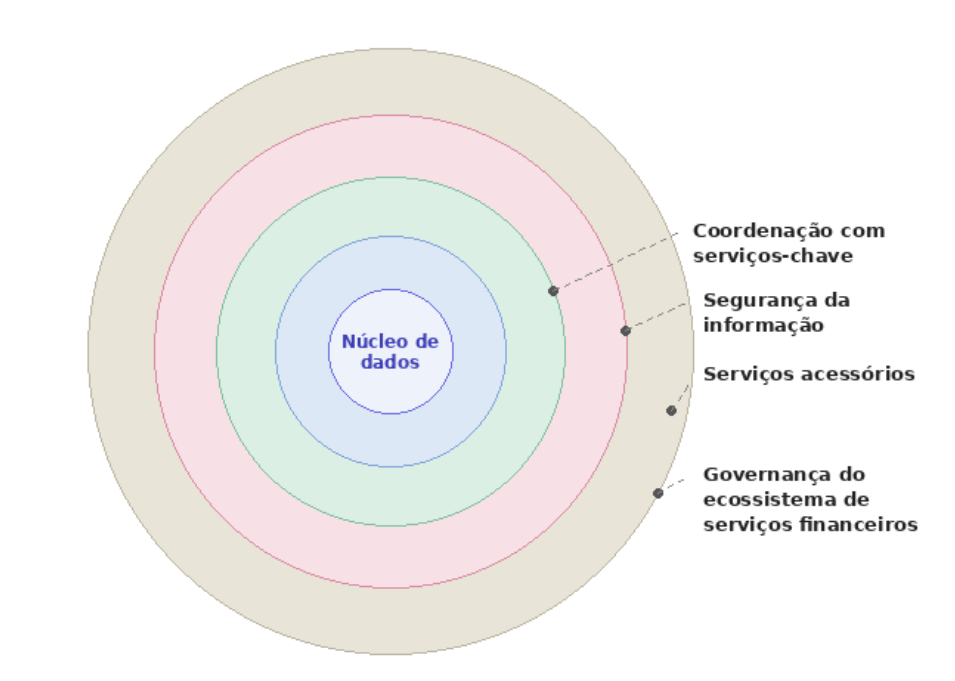
\includegraphics[width=\textwidth]{assets/figura_1_bancos_independentes.png}
    \label{fig:bancos_independentes}
\end{figure}

Para concretizar essa visão, pensamos um núcleo de armazenamento e distribuição baseada em \textit{containers} Docker. A etapa de aquisição de dados, implementada de forma independente por Evamberto Oliveira, executa o \textit{MetaTrader 5} integrado a provedores externos, como as corretoras Rico, XP e Inter. Esses contêineres de extração (mt5BRIDGE) enviam os dados dos ativos para um canal da API de armazenamento do qDATA, que os persiste no banco de dados. Toda a ingestão ocorre via Representational State Transfer (REST)/HTTPS, justificável pelo fluxo relativamente baixo de entrada de dados, o que evidencia a coordenação necessária entre o mt5BRIDGE e o qDATA.

A persistência no qDATA é gerenciada por um banco de dados PostgreSQL com estratégia de \textit{Upsert} (Update + Insert). Essa abordagem previne duplicidades e mantém a consistência das informações mesmo sob alta taxa de ingestão simultânea. Ademais, o armazenamento é otimizado para séries temporais por meio do uso de hyper-tabelas da extensão TimeScale.

No que tange à distribuição técnica dos dados, o protocolo \textit{gRPC Remote Procedure Call} (gRPC) permite o estabelecimento de conexões contínuas (com sessão) e uma obtenção mais rápida, sendo útil em consultas massivas, como o resgate de dados correspondentes a um ano inteiro. Contudo, visando complementar e facilitar essa distribuição, implementou-se também uma interface HTTPS/2. Essa segunda opção foi projetada para que a conexão com a API pudesse ser realizada de forma mais ágil pelos usuários (pesquisadores e desenvolvedores), uma vez que o uso de HTTPS apresenta uma curva de aprendizado substancialmente menor e um \textit{overhead} de desenvolvimento reduzido.

À medida que a ferramenta avançou em produção, membros do projeto passaram a utilizá-la como base para construir serviços quantitativos auxiliares, tais como cálculos de correlações com \textit{bootstrapping}, experimentos em Python de trabalhos teóricos conduzidos no projeto, e rotinas de identificação de anomalias. Esse cenário reforça o desenho de um ecossistema coeso de serviços e análises de apoio.

Por fim, cabe ressaltar que a plataforma qDATA é uma ferramenta de uso estritamente interno ao Laboratório de Tecnologias Inovadoras (LTI) e à comunidade de pesquisa da Universidade Federal do Ceará. Ela não configura um serviço comercial de distribuição de dados de mercado para terceiros externos. Assim, estabelecemos uma rigorosa política de não revenda, não sublicenciamento e não disponibilização pública dos dados obtidos. Essa segurança reflete-se no gerenciamento granular de permissões de acesso em um banco de dados específico. A implantação de contêineres individuais para aquisição de dados será, futuramente, discutida com o responsável pelo mt5BRIDGE.

A arquitetura do ecossistema de microsserviços promove o princípio de \textbf{Separação de Responsabilidades} (\textit{Separation of Concerns}): o qDATA concentra-se exclusivamente no fornecimento dos dados como serviço compartilhado, enquanto as ferramentas dos pesquisadores — painéis analíticos, algoritmos de ordens de \textit{trading} e modelos estatísticos — focam em suas lógicas específicas. Isso elimina acoplamentos indesejados e permite que diferentes membros do LTI e projetos da UFC utilizem essa infraestrutura de dados sem redundâncias.

\begin{figure}[htb]
    \centering
    \caption{Visão geral da arquitetura: Ingestão distribuída e distribuição segura de dados financeiros.}
    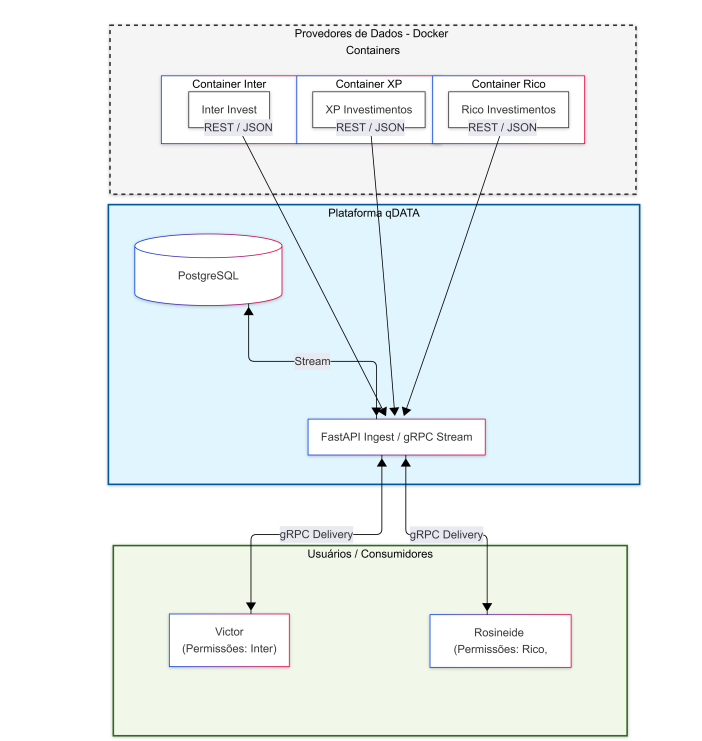
\includegraphics[width=\textwidth]{assets/figura_2_visao_arquitetura.png}
    \label{fig:visao_arquitetura}
\end{figure}

Deve-se observar, no entanto, que o uso em outros projetos requer, por questões legais e de governança, a execução de uma nova instância isolada do sistema, haja vista as restrições à distribuição. Nesse contexto de separação de responsabilidades, a execução de ordens de compra e venda, por exemplo, permanece uma tarefa local e autônoma de cada ferramenta consumidora, sem interferência direta com a camada de ingestão remota ou de distribuição de dados. Tanto por questões legais quanto de engenharia de software, decidiu-se consolidar o ecossistema sob o escopo do \textit{LTI FinHub}.

O acesso à plataforma é protegido por autenticação baseada em \textit{JSON Web Token} (JWT) integrada ao Supabase, viabilizando um controle de acesso granular por perfil de usuário e por provedor de dados. Dessa forma, o trabalho aqui apresentado descreve a concepção, a arquitetura e a implementação dessa infraestrutura de dados, avaliando sua contribuição para as atividades do LTI e a viabilidade do uso da ferramenta em outros projetos da UFC.

\begin{figure}[htb]
    \centering
    \caption{Diagrama de consumo e execução: Autonomia dos pesquisadores e separação de responsabilidades.}
    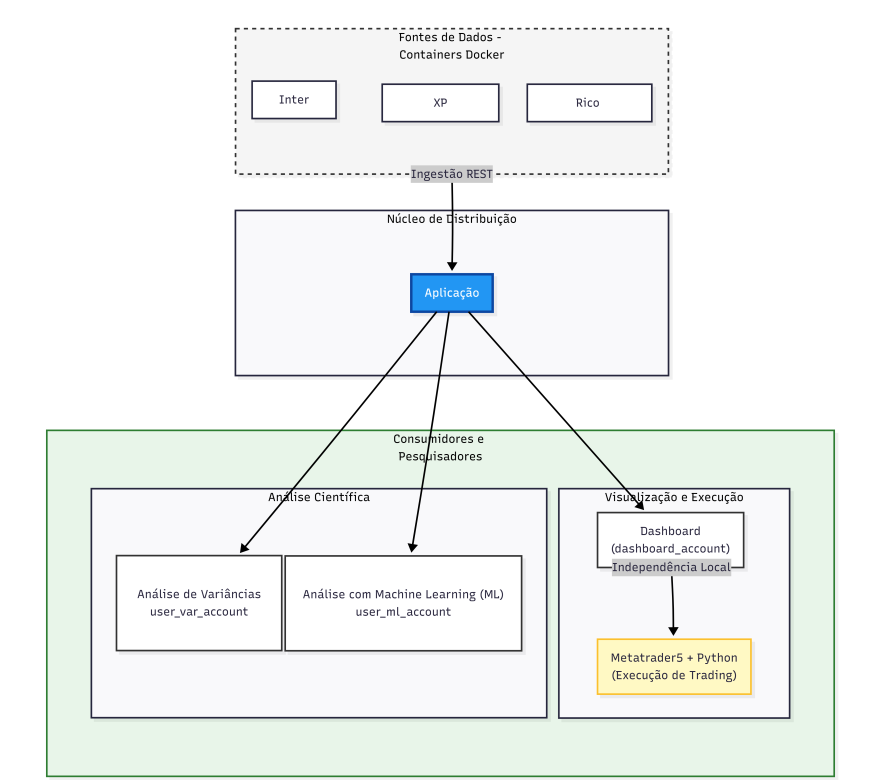
\includegraphics[width=\textwidth]{assets/figura_3_autonomia_pesquisadores.png}
    \label{fig:autonomia_pesquisadores}
\end{figure}

\section{Escopo}

A plataforma qDATA abrange a ingestão de dados de corretoras selecionadas, o armazenamento e a distribuição desses dados para consumidores internos do grupo de pesquisa LTI, com foco no projeto \textit{Análise de Séries Financeiras}. Dentro do escopo técnico estão a comunicação com um software de aquisição de barras \textit{Open, High, Low, Close} (OHLC), o armazenamento otimizado com hyper-tabelas através do TimeScale — o que viabiliza a entrega de dados em alta velocidade aos consumidores autorizados — e a disponibilização desses dados via HTTPS, visando cenários que exigem praticidade e agilidade no desenvolvimento de aplicações.

Ao longo deste trabalho, também são analisadas as políticas de acesso a dados, o registro e ativação de usuários, o gerenciamento de contas do projeto e outras questões de segurança que impactam diretamente a ferramenta qDATA e o ecossistema como um todo. Assim, partindo da ferramenta qDATA como elemento central, o escopo se expande radialmente para uma visão arquitetural mais ampla, englobando o apoio à governança de TI do projeto \textit{LTI Finanças}.

\begin{figure}[htb]
    \centering
    \caption{Demandas do núcleo de dados.}
    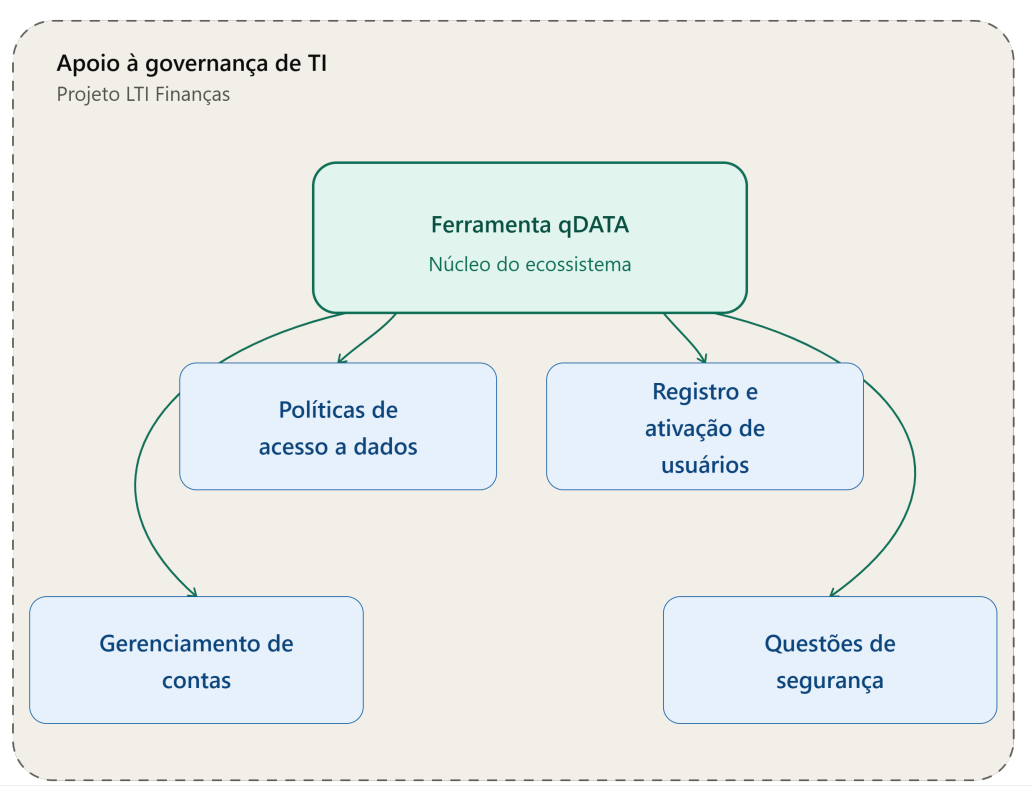
\includegraphics[width=\textwidth]{assets/figura_4_demandas_nucleo.png}
    \label{fig:demandas_nucleo}
\end{figure}

Por outro lado, estão categoricamente fora do escopo desta plataforma: a execução de ordens de compra e venda nas corretoras, a gestão de risco financeiro e o desenvolvimento de interfaces de \textit{trading} para usuários finais. O qDATA atua exclusivamente como infraestrutura de dados compartilhada, cabendo à lógica de análise e negociação permanecer sob a estrita responsabilidade de cada ferramenta ou pesquisador consumidor.

\section{Objetivos}

\subsection{Objetivo Geral}

Projetar e implementar uma plataforma de dados financeiros centralizada e orientada à disponibilidade para o projeto \textit{Análise de Séries Financeiras} do LTI.

\subsection{Objetivos Específicos}

\begin{itemize}
    \item Integrar a plataforma com os \textit{containers} Docker de aquisição de dados do MetaTrader 5 (MT5), os quais operam em ambiente Linux utilizando Wine;
    \item Desenvolver o núcleo de ingestão e armazenamento de dados empregando o \textit{framework} FastAPI e o banco de dados PostgreSQL, mediado por protocolo HTTPS REST;
    \item Implementar serviços de distribuição de dados aos consumidores utilizando o protocolo gRPC;
    \item Disponibilizar uma interface HTTPS análoga ao serviço gRPC, provendo \textit{endpoints} mais amigáveis e flexíveis para desenvolvedores iniciantes ou colaboradores que priorizam agilidade de prototipagem;
    \item Integrar a arquitetura a um sistema de autenticação e autorização via Supabase e JWT, viabilizando um controle de acesso granular que diferencia permissões de leitura e gravação através de um atributo de modo de usuário;
    \item Estabelecer mecanismos iniciais para a garantia de disponibilidade, abrangendo a implementação de testes unitários (via \texttt{pytest}) e o planejamento de fluxos de integração contínua (GitHub Actions), que utilizam estes testes.
    \item Implementar um ambiente de \textit{staging} em nosso servidor
    \item Validar a robustez da plataforma com consumidores reais do LTI por meio da alimentação do \textit{dashboard} analítico;
    \item Comparar o desempenho das interfaces de distribuição (gRPC, gRPC-Web e HTTPS) em termos de latência e consumo de banda, gerando histogramas para avaliação da variância métrica;
    \item Documentar formalmente as políticas de controle de acesso e versionamento como prática basilar de governança de TI;
    \item Analisar e definir as restrições de \textit{compliance} pertinentes ao uso e à distribuição interna dos dados financeiros coletados.
\end{itemize}

\section{Organização do Trabalho}

Este trabalho está organizado em seis capítulos, incluindo esta introdução. O Capítulo 2 aborda a fundamentação teórica que dá suporte às decisões de \textit{design} e às tecnologias empregadas na plataforma. O Capítulo 3 descreve, de modo pragmático, a metodologia adotada para o desenvolvimento do projeto. O Capítulo 4 apresenta o cronograma das atividades. O Capítulo 5 detalha os resultados técnicos, organizacionais e de adoção obtidos ao longo do trabalho. Por fim, o Capítulo 6 traz a conclusão, delineando as considerações finais e os possíveis trabalhos futuros.

\chapter{FUNDAMENTAÇÃO TEÓRICA}

Este capítulo tem como objetivo apresentar os conceitos teóricos, padrões arquiteturais e tecnologias que embasam o desenvolvimento da plataforma qDATA. Ao longo das próximas seções, discutiremos as bases fundamentais necessárias para a compreensão das escolhas metodológicas detalhadas posteriormente, contextualizando-as no cenário de engenharia de software voltada a sistemas de alta disponibilidade e baixa latência.

Dada a natureza do problema do LTI, que exige a ingestão contínua de grandes volumes de dados financeiros (barras OHLC) e seu consumo em atividades internas do LTI, a infraestrutura projetada baseia-se fortemente em práticas modernas da indústria. Discorreremos sobre como conceitos consolidados, como microsserviços, conteinerização e comunicação híbrida via protocolos eficientes, sustentam os requisitos operacionais sem comprometer a estabilidade do serviço.

\section{O Ecossistema LTI FinHub}

O FinHub é um ecossistema abrangente desenvolvido no âmbito do Laboratório de Tecnologias Inovadoras (LTI). Trata-se de um sistema amplo que orquestra múltiplos serviços e componentes para viabilizar a pesquisa quantitativa avançada. A Figura \ref{fig:ecossistema_finhub} ilustra a arquitetura conceitual e a interação entre os diversos elementos que compõem este ambiente.

Neste trabalho, adotamos como ponto de partida inicial o componente qDATA, dedicando a ele um enfoque predominantemente técnico. Contudo, conservamos a perspectiva sistêmica de que o qDATA, embora seja um componente individual, desempenha um papel central e, portanto, precisa se relacionar adequadamente com os demais serviços do ecossistema. O sucesso de sua implementação depende da interoperabilidade harmoniosa com módulos como o \textit{feeder}, os painéis de visualização (\textit{dashboards}) e os futuros serviços de simulação.

Ademais, ressalta-se que o presente estudo consolida as bases infraestruturais. Um trabalho futuro (TCC2) dará ênfase a aspectos mais amplos, como governança de TI, aprofundamento na arquitetura de microsserviços e práticas de \textit{Product Ownership}, garantindo que a evolução do ecossistema FinHub ocorra de forma gerenciada, escalável e alinhada às necessidades estratégicas dos pesquisadores envolvidos.

\begin{figure}[htb]
    \centering
    \caption{Ecossistema LTI FinHub}
    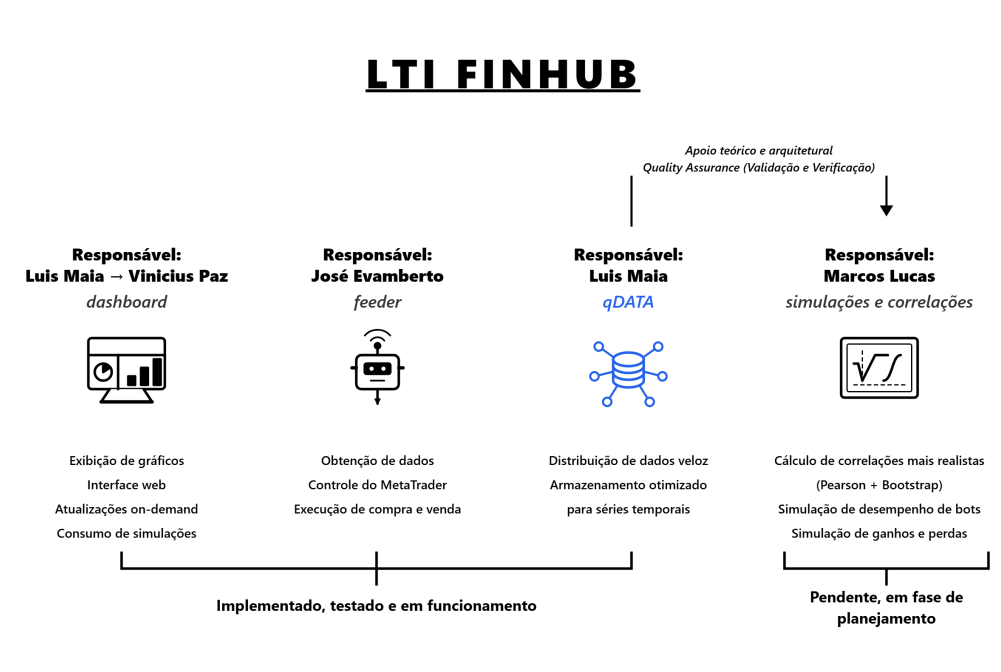
\includegraphics[width=\textwidth]{assets/figura_5_ecossistema_finhub.png}
    \label{fig:ecossistema_finhub}
\end{figure}

\section{Arquitetura de Microsserviços}

A arquitetura de microsserviços consiste em uma abordagem na qual uma única aplicação é composta por um conjunto de pequenos serviços, cada um executando seu próprio processo e comunicando-se por meio de mecanismos leves, geralmente \textit{Application Programming Interfaces} (APIs) sobre o protocolo \textit{Hypertext Transfer Protocol} (HTTP). Conforme postulado por \citeonline{newman2015building}, essa arquitetura enfatiza serviços independentemente implantáveis, construídos em torno de capacidades de negócios e com implantação automatizada.

\begin{comment}
Ao contrário de abordagens monolíticas — onde todos os componentes lógicos (interface, regras de negócio e acesso a dados) são empacotados juntos —, os microsserviços promovem um acoplamento fraco e alta coesão. Essa granularidade permite que equipes operem de forma descentralizada, atualizando um componente sem o risco de impactar a disponibilidade geral do sistema. Na engenharia de software para plataformas financeiras, a resiliência gerada pelo isolamento de falhas é de extrema importância.
\end{comment}

Ao contrário de abordagens monolíticas – onde todos os componentes lógicos (interface, regras de negócio e acesso a dados) são desenvolvidos dentro de um mesmo repositório – os microsserviços promovem um acoplamento mais fraco, e melhora a coesão. Evidentemente, essa melhoria não é absoluta, pois o desmembramento de um software grande em unidades menores pode impactar contratos, dependências, segurança ou a integração com outros serviços. Ainda assim, as vantagens citadas ultrapassa a mera organização arquitetural do código. 

Nesse sentido, conforme visto nos trabalhos dentro do laboratório, tal abordagem permitiu mais flexibilidade para a equipe, e membros da equipe podem se voluntariar a serem responsáveis por um componente específico. Uma prática interessantíssima nesse cenário é a atribuição a um membro de responsabilidade "end-to-end" por algum(s) serviço(s). Em outras palavras, é possível estruturar a organização do laboratório de modo que certos colaboradores sejam totalmente responsáveis por um serviço. Tal trabalho é, ainda, viabilizado pelo tamanho do serviço, que devido à modularização não representa um software inteiro, mas apenas um parte do todo.

No contexto deste trabalho, a arquitetura de microsserviços justifica a divisão estrutural entre o componente de coleta de dados (\textit{feeder}) e a plataforma centralizadora (qDATA). Ou seja, foi projetado para que as responsabilidades de (1) aquisição das séries temporais e de (2) armazenamento e distribuição sejam escaladas, monitoradas e mantidas de maneira totalmente autônoma.

Nesse contexto, destaca-se que uma versão inicial – e precária – do \textit{feeder} foi prototipada e usada em experimentos no projeto, mas a versão final e de qualidade só foi desenvolvida posteriormente, pelo discente José Evamberto Lima Oliveira, conforme descrito em seu trabalho \textit{Manutenção e Evolução do Sistema MT5-Websocket-Bridge no projeto de extensão LTI – Análise de séries financeiras} \cite{oliveira2026}.

\section{Coleta de Dados com Tickers Especializados}

A especialização em coleta de dados, por parte do discente José Oliveira, cujo trabalho se comunica diretamente com o meu, abriu caminho para três possibilidades de trabalho. Em primeiro lugar, possibilitou a divisão da carga de trabalho, permitindo que o trabalho do sistema de dados fosse dividido em duas partes menores, evitando a sobrecarga laboral.

Em segundo lugar, tornou possível a coleta especializada de tickers. Nesse sentido, cita-se o fato de que há dois tipos de tickers na biblioteca Python do Metatrader5. São eles: (1) \texttt{mt5.COPY\_TICKS\_TRADE}, que filtra a base de dados do MT5 e só te entrega os momentos em que um comprador e um vendedor fecharam negócio.

Em segundo lugar, temos o (2) \texttt{mt5.COPY\_TICKS\_INFO}, que traz apenas as atualizações do Book de Ofertas (Livro de Preços). Ou seja, alguém colocou, moveu ou cancelou uma ordem limite de compra (Bid) ou venda (Ask), mas nenhum negócio foi fechado. Ele é fortemente recomendado para trabalhos estatísticos, simulações, uso em estratégias de \textit{trading}, etc.

Por fim, temos o tipo de ticker (3) \texttt{mt5.COPY\_TICKS\_ALL} que traz absolutamente tudo. Cada vez que o Bid mudou, o Ask mudou, ou um negócio aconteceu, uma nova linha é gerada. Deve-se notar que o volume de dados gerado por essa flag é gigantesco, especialmente em ativos líquidos como mini-índice (WIN), um tipo ideal para trabalhos e técnicas estatísticas que dependem muito de volume.

Nesse contexto, no que tange aos \textit{stakeholders} do projeto, temos a possibilidade de ofertar à equipe e à coordenadora do projeto três tipos diferentes de dados para um mesmo ativo, que devem ser escolhidos conforme a necessidade de cada demanda. Concluindo, o trabalho realizado em cada um desses componentes se torna mais especializado, produzindo componentes de mais qualidade no produto final.

\section{Contêineres e Docker}

A conteinerização revolucionou a implantação de software ao oferecer uma virtualização em nível de sistema operacional (processo). O Docker despontou como a principal ferramenta para essa prática, permitindo que desenvolvedores empacotem uma aplicação com todas as suas dependências, bibliotecas e arquivos de configuração necessários em um único artefato portável \cite{merkel2014docker}.

Um dos maiores ganhos operacionais da utilização de contêineres é o princípio conhecido como "\textit{build once, run anywhere}" (construa uma vez, execute em qualquer lugar). Na prática, se o contêiner funciona no ambiente de desenvolvimento, seu comportamento será idêntico nos ambientes de teste, homologação e produção, erradicando a clássica síndrome do "na minha máquina funciona". Essa previsibilidade minimiza substancialmente o esforço logístico em implantações complexas.

No desenvolvimento do projeto, o Docker permite empacotar o código do banco de dados e o código do ASGI (FastAPI) sem expor a máquina hospedeira a configurações conflitantes, além de permitir rápida manutenção do banco de dados e \textit{deploys} mais seguros.

\subsection{Compatibilidade de Binários em Ambientes Linux (Wine)}

Ainda dentro do domínio da infraestrutura de contêineres, surge frequentemente a necessidade de compatibilizar binários compilados exclusivamente para a plataforma Windows em ambientes operacionais baseados em Linux. O MT5, terminal frequentemente mandatório para conexão com corretoras brasileiras (como XP, Rico e Clear), possui versões nativas unicamente para o ecossistema da Microsoft.

Para contornar tal barreira no Linux, convenciona-se utilizar a camada de compatibilidade Wine (\textit{Wine Is Not an Emulator}). Trata-se de um software que traduz as chamadas de sistema (API) do Windows para equivalentes no padrão \textit{Portable Operating System Interface} (POSIX) do Linux em tempo real, evitando os atrasos de desempenho característicos de emuladores convencionais ou máquinas virtuais pesadas \cite{winehq2026}.

\section{Separação de Preocupações (Separation of Concerns)}

O princípio da Separação de Preocupações, originário dos primórdios da Ciência da Computação, determina que um sistema deve ser estruturado em seções distintas, onde cada seção lida com um conjunto específico e delineado de informações e tarefas. Um módulo deve ter uma, e apenas uma, razão primária para sofrer modificações.

Em sistemas distribuídos modernos, aplicar esse princípio significa evitar componentes "Deus", isto é, objetos ou serviços que sabem e fazem demais, um fenômeno discutido nas aulas de Programação Orientada a Objetos. Ao delegar as preocupações de obtenção de dados de mercado para um sistema dedicado, libera-se a ferramenta consumidora da tarefa de gerenciar autenticações complexas de API ou manter a resiliência de \textit{sockets} contínuos, focando unicamente na análise dos dados em si. Mais do que isso: essa arquitetura permitiu delegar a responsabilidade do "Departamento de Aquisição de Dados" (figura de linguagem) a um gerente dedicado especificamente a isso.

No domínio do Laboratório de Tecnologias Inovadoras, a adoção incisiva deste conceito molda a justificativa central do trabalho. O qDATA concentra-se puramente em agir como infraestrutura de dados compartilhada (\textit{Market Data}). A lógica de análise quantitativa, o treinamento de modelos estocásticos e a execução de ordens nas corretoras permanecem estritamente sob responsabilidade do cliente (\textit{researcher}). Essa fronteira rígida protege o núcleo do sistema de \textit{bugs} advindos de modelos preditivos em fase de experimentação.

\section{Protocolos de Comunicação: REST/HTTP e gRPC}

A intercomunicação eficaz é o coração de qualquer arquitetura de serviços distribuídos. O REST (\textit{Representational State Transfer}), introduzido por \citeonline{fielding2000}, tornou-se o padrão \textit{de facto} na web, caracterizado por sua operação \textit{stateless} sobre HTTP e pela ampla adoção global por sua clareza de uso. Contudo, em virtude de tradicionalmente carregar respostas verbosas em texto \textit{JavaScript Object Notation} (JSON) e depender de conexões repetidas no HTTP/1.1, a comunicação REST costuma esbarrar em gargalos quando exigida baixa latência e alta vazão (milhões de eventos por minuto).

Em contrapartida, o gRPC (\textit{gRPC Remote Procedure Call}) é um \textit{framework} moderno, focado em alta performance, que utiliza o protocolo HTTP/2 subjacente e o formato de serialização binária Protocol Buffers (Protobuf). Ele viabiliza não apenas chamadas incisivamente menores e mais rápidas no envio por rede, como também introduz o conceito valioso de conexões multiplexadas e o \textit{streaming} bidirecional de mensagens contínuas, mantendo o canal perenemente aberto \cite{google2016grpc}. Em outras palavras, conseguimos enviar múltiplas requisições por um mesmo canal \textit{Transmission Control Protocol} (TCP) em paralelo de um ponto de vista lógico, aumentando a performance da rede, e delegando a responsabilidade de controle de fluxo para o protocolo HTTP/2, que é otimizado para esse tipo de comunicação.

Adotamos, portanto, uma arquitetura de rede híbrida alinhada com as melhores práticas da indústria financeira. A ingestão de barras (\textit{feeder} enviando ao núcleo) ocorre via \textit{endpoints} REST baseados no HTTP clássico, permitindo fácil inspeção, monitoramento com \textit{webhooks} e integração simplificada. Simultaneamente, a distribuição dos dados temporais para o painel (\textit{dashboard}) dos pesquisadores é trafegada via canais gRPC otimizados, superando obstáculos inerentes ao JSON e minimizando fortemente a latência nas consultas volumosas de cotações históricas. Esclarecemos que a melhoria feita ao usar Protocol Buffers (Protobuf) em vez de JSON consiste no fato que esse tipo de serialização é mais compacta, além de ser mais rápida para serializar e desserializar em comparação ao formato de texto (JSON, \textit{Extensible Markup Language} (XML), etc). Nesse sentido, definimos serialização e desserialização como o processo de converter um objeto entre um formato utilizável pela memória do computador e um formato utilizável para transmissão ou armazenamento.

\section{Bancos de Dados para Séries Temporais: TimescaleDB}

Dados financeiros em formato OHLC (\textit{Open, High, Low, Close}) apresentam o caráter uníssono e linear de séries temporais (\textit{time-series}). Os bancos de dados relacionais tradicionais, embora robustos nas consultas transacionais simples e cruzamentos complexos (JOINs), frequentemente demonstram acentuada degradação em desempenho e crescimento descontrolado no espaço de armazenamento físico à medida em que as tabelas acumulam centenas de milhões de pontos sequenciais de observação no tempo.

A extensão de Postgres denominada "TimescaleDB" se projeta essencialmente como uma ferramenta voltada à adequação do Sistema de Gerenciamento de Banco de Dados (SGBD) padrão PostgreSQL aos exigentes critérios de \textit{Time-Series Data}. Seu principal diferencial repousa nas chamadas \textit{hypertables}: na superfície atuam identicamente como tabelas relacionais clássicas, no entanto operam no interior criando e gerenciando o particionamento dinâmico automático em blocos temporais isolados \cite{timescale2017}.

Desta forma, os pesquisadores do LTI podem submeter requisições envolvendo densas estatísticas com cálculos de médias e consolidação dos volumes intradiários em escalas cronológicas maiores (através das funções nativas como \texttt{time\_bucket}). O mecanismo subjacente somente inspeciona as frações de dados contidas nos intervalos requeridos (sem necessidade de percorrer todos os registros contidos em base de dados), e utiliza ainda algoritmos de compressão columnar sofisticados que propiciam economia substancial do espaço em disco sem sacrifício da presteza das consultas.

\section{FastAPI e Programação Assíncrona (ASGI)}

Com o advento e adoção crescente de ambientes concorrentes de \textit{Input/Output} (I/O), o padrão Python \textit{Asynchronous Server Gateway Interface} (ASGI) (\textit{Asynchronous Server Gateway Interface}) ascendeu para solucionar o bloqueio síncrono que assolava seus antecessores (como o Web Server Gateway Interface). O padrão ASGI gerencia requisições paralelamente de forma assíncrona, o que significa que a \textit{thread} do servidor pode atender a outras chamadas web sem travar a execução enquanto aguarda por respostas de tráfego de redes externas ou resoluções de consultas morosas no banco de dados.

O \textit{framework} FastAPI constrói-se exatamente sob essa base arquitetural assíncrona, ancorando suas credenciais de escalabilidade. Notabilizado pelo elevado e provado desempenho — equiparável a \textit{frameworks} baseados em Node.js e até mesmo linguagens compiladas como Go —, o FastAPI inclui documentação automatizada nativa (Swagger UI e ReDoc), e integra de maneira transparente a validação estrita de parâmetros das rotas por meio do robusto ecossistema de validação e tipagem "Pydantic" \cite{ramirez2018fastapi}.

Na engenharia do qDATA, essa capacidade de escalar perante tráfego denso foi determinante na seleção do FastAPI para hospedar a camada REST \textit{controller} do microsserviço central. O fluxo ininterrupto de dezenas (ou centenas) de \textit{feeders} simultâneos despejando as atualizações do índice a cada minuto causaria um enfileiramento nocivo numa estrutura web linear, ao passo que em regime assíncrono o banco de dados e a rede resolvem as requisições recebidas com sobreposição altamente otimizada. Cabe destacar que embora o serviço de distribuição de dados tenha sido feito com gRPC, a alimentação dos dados foi implementada via \textit{endpoints} REST/HTTP de recepção de dados. Essa escolha foi feita por questões de tempestividade do projeto, além do fato de que o gargalo desse ecossistema é a distribuição, e não a ingestão.

\section{Estratégia de Upsert e Idempotência}

Sistemas distribuídos convivem invariavelmente com o modelo de entrega na rede conhecido como "pelo menos uma vez" (\textit{at-least-once}), o que indica que repetições não intencionais de requisições ou atrasos são corriqueiros mediante instabilidades de conectividade. Para ingerir ininterruptamente um extenso número de barras de ativos e neutralizar os duplos envios na rede ou reconexões espontâneas do \textit{feeder}, não basta contar puramente com validações lógicas na camada da aplicação do servidor. É imperativa uma lógica sistêmica de banco de dados para prevenção à duplicação de anomalias temporais.

O mecanismo de \textit{Upsert} constitui o ato conjugado e atômico de inserir um registro se este for perfeitamente novo na persistência e, em oposição, efetuar estritamente uma atualização no registro já contido caso este fira metadados imutáveis pré-condicionados (as chaves concorrentes primárias). No dialeto moderno do banco de dados PostgreSQL, invoca-se essa característica via instrução \texttt{INSERT ON CONFLICT DO UPDATE}. Neste projeto, isso foi feito utilizando a função \texttt{merge} do \textit{Object-Relational Mapping} (ORM) (Object-Relational Mapping) do SQLAlchemy. Essa mescla transacional provê atualização sem carecer empenhar dispendiosos travamentos de linha (\textit{row locks}) longos no processo.

Para que as consultas gRPC entreguem aos painéis dos pesquisadores gráficos perfeitamente sincronizados, isentos de contaminações das séries e saltos matemáticos fictícios, os barramentos de injeção aplicam em profundidade este corolário. Na eventualidade de os \textit{feeders} retransmitirem parcelas horárias previamente já introduzidas, a abordagem \textit{Upsert} consolida a consistência atômica. É, portanto, garantida a premissa de \textit{Idempotência}: requisições idênticas com os mesmos parâmetros reproduzirão exatamente a mesma resultante estável a despeito das eventuais repetições impostas pelo emissor.

\section{Autenticação e Autorização com JWT e Supabase}

Garantir o livre mas vigiado intercâmbio de dados de mercado requer o uso de robustos arcabouços de gestão de identidade e acesso entre sistemas. O token JWT (\textit{JSON Web Token}) fornece a assinatura unificada baseada em um corpo de formato JSON codificado que detém asserções (\textit{claims}) prévias. Tais \textit{claims} validam a legitimidade sem impor onerosas revisões sistêmicas (pesquisas na tabela de sessão do banco) em cada requisição transacionada via rede, seguindo fidedignamente o padrão aberto da indústria formulado no \textit{Request for Comments} (RFC) 7519 do \textit{Internet Engineering Task Force} (IETF) \cite{rfc7519}. Em outras palavras, realizamos autenticação utilizando processamento lógico, em vez de consulta a um banco de dados, o que é mais eficiente e escalável. Notavelmente, a obtenção de um JWT válido, um processo que é feito apenas uma vez por sessão, envolve um banco de dados. Isto não é problemático, pois uma sessão pode durar horas ou dias, conforme o critério do engenheiro que desenhou as configurações do JWT. Haja vista que o domínio do presente trabalho se concentra em redes, sistemas distribuídos, e dados financeiros, utilizamos uma solução de nível mais alto e maior simplicidade para lidar com o manejo e autenticação dos usuários. Mais especificamente, utilizamos o Supabase para gerenciar quem tem permissão para receber um token JWT válido.

Dessa forma, esses \textit{tokens} são distribuídos por um \textit{Backend as a Service} (BaaS) (\textit{Backend as a Service}) \cite{supabase2020}. A implementação futura de Políticas de Segurança Orientadas a Linhas (\textit{Row Level Security} - RLS) do PostgreSQL aliado ao gerenciamento contínuo das credenciais — sem sobrecarregar nosso código próprio de engenharia com tratamento complexo de senhas — representa o estado da arte das soluções para gerência de perfis e controle de acesso seguro.

Com essa proteção validada e autossuficiente via JWT, as interações entre os variados pesquisadores e o grupo diretor principal do LTI ganham controles finamente ajustados de permissão e isolamento granular. Ao invés da tradicional adoção de um gargalo de API Gateway obsoleto centralizando a autorização primária de forma bloqueante, os próprios microsserviços atestam localmente de forma criptográfica (na verificação de chaves assimétricas públicas) a permissão adequada requerida para leitura do \textit{streaming} das cotações.

\section{Desenvolvimento Incremental e Integração Contínua}

Em contraponto às abordagens metodológicas clássicas e estritas de Cascata, metodologias contemporâneas ágeis pregam os aprimoramentos graduais focados em validação rápida ao invés do dispêndio excessivo na abstração estática e antecipada do projeto. A essência do Desenvolvimento Incremental consiste no adorno iterativo de pequenos recursos (ou subcomponentes funcionais da aplicação) dispostos contínua e ordenadamente sobre uma fundação com forte padronização contratual nas interfaces de comunicação do sistema. Admito que uma preocupação quanto à Engenharia de Software é a possibilidade de que o desenvolvimento incremental se reduza ao mero trabalho \textit{ad-hoc}.

No entanto, os avanços em ferramentas de linguagem natural têm avançado o desenvolvimento incremental a partir da criação de planos detalhados com mais facilidade, tanto antecipando problemas arquiteturais quando apontando ou criando possibilidades para evolução. Essa maleabilidade análise técnica do código e codificação aumentada (\textit{augmented coding}), evoluíram a prática de \textit{Continuous Integration} / Integração Contínua (CI). No mais, conforme a disponibilidade de tempo, uma lista de tarefas simples (\textit{task list}) pode ser utilizada para determinar (especificar) a utilização de algumas técnicas de engenharia, tal como requerer a construção de um Diagrama de Classes bem feito para representar a estrutura do código, um Diagrama de Atividades para especificar o processo de autenticação e consumo de dados, e um Diagrama de Sequência, que é mais crítico, para representar a interação entre os micro-serviços do ecossistema. Tem se tornado mais claro que este último diagrama seria crítico, pois no início do projeto tínhamos apenas o qDATA, o \textit{feeder} e o \textit{dashboard}, porém durante a criação deste TCC emergiu no LTI a necessidade de um micro-serviço de simulação de correlações \textit{bootstrapped}.

Esse novo cenário abre margem para a consolidação do uso de estratégias de orquestração de múltiplos repositórios (como submódulos e ferramentas de governança de código), um diferencial crucial no que tange à garantia de intercompatibilidade versional e à construção sustentável de ecossistemas de microsserviços. No Git, isso é feito com a função de submódulos, usando o comando \texttt{git submodule add} para adicionar um repositório dentro de outro. O submódulo é uma referência a um \textit{commit} específico do repositório externo, e o Git mantém o controle dessa referência. Assim, quando alguém clona o repositório principal, ele pode usar o comando \texttt{git submodule update --init --recursive} para baixar os submódulos e garantir que as versões corretas sejam usadas.

Dessa forma, a adoção de um \textit{pipeline} de CI robusto e automatizado, utilizando ferramentas como GitHub Actions, Jenkins ou GitLab CI/CD, é imperativa para o sucesso do projeto. O \textit{pipeline} deve incluir etapas de construção, testes automatizados (unitários, de integração e de regressão), análise estática de código e validação de segurança. Isso assegura que cada alteração no código seja rigorosamente verificada antes de ser integrada ao ramo principal, mantendo a estabilidade e a qualidade do sistema à medida que ele evolui. Como dito antes, tal fato não era tão evidente no estado inicial do ecossistema, pois existem apenas três aplicações: (1) qDATA, (2) MT5-Websocket-Bridge, e (3) o \textit{dashboard}. Todavia, à medida que o projeto cresce e mais componentes são adicionados – como o (4) Serviço de Simulações com Bootstrapping – a importância de um \textit{pipeline} de CI bem estruturado se torna ainda mais crítica para garantir a coesão e a integridade do sistema como um todo.

\chapter{METODOLOGIA}

A metodologia adotada neste trabalho foi estruturada para orientar o desenvolvimento de uma plataforma centralizada de recepção e distribuição de dados financeiros para o Laboratório de Tecnologias Inovadoras (LTI), com ênfase em baixa latência, disponibilidade. O estudo combina investigação bibliográfica, definição de requisitos a partir de um problema real do laboratório, desenvolvimento incremental da solução e proposta de validação por meio de testes funcionais e experimentos quantitativos.

\section{Visão geral da metodologia}

O ponto de partida desta pesquisa é a necessidade de responder à questão proposta anteriormente: como fornecer, de forma centralizada, sem dependências do MT5 e com baixa latência, dados em tempo real e históricos do ativo Mini-Índice Ibovespa para os pesquisadores do LTI ? A partir desse problema, a metodologia foi organizada como um processo prático e iterativo, no qual a arquitetura da solução e dos experimentos, as implementações técnicas e os testes de validação evoluem em conjunto.

Em vez de assumir um planejamento rígido e integral desde o início, como por exemplo um planejamento do tipo cascata, a proposta admite a incorporação gradual de requisitos e ajustes técnicos decorrentes das demandas advindas dos consumidores e das necessidades técnicas supervenientes. Tal dinamicidade exige, notavelmente, que haja um grau adequado de padronização de interfaces \textit{back-end} e camadas-\textit{controller} de dados no que diz respeito à API da plataforma.

Para além de questões de integração, esse \textit{framework} é adequado porque muitos requisitos funcionais advêm de demandas de usuários reais do laboratório. Tais demandas, frequentemente, não são de conhecimento dos engenheiros. Em outras palavras, nós não temos pleno conhecimento do domínio-técnico ou domínio-funcional. Neste estudo, tal domínio consiste principalmente de estatística avançada, redes neurais e processos estocásticos. Assim, a metodologia visa um gerenciamento de projeto flexível o suficiente para acomodar diferentes necessidades, mas também suficientemente determinística para garantir a operabilidade contínua do ecossistema de serviços (\textit{feeder}, qDATA, \textit{dashboard}, etc).

\section{Questões de pesquisa}

Com base na pergunta principal do trabalho, foram definidas as seguintes questões de pesquisa, mais aderentes ao contexto do LTI:
\begin{enumerate}
    \item Como estruturar uma infraestrutura única e pública de dados financeiros a qual elimine ou reduza a necessidade de dependências de aquisição de dados (MT5, Polygon, etc)?
    \item Quais componentes arquiteturais, protocolos de rede e \textit{frameworks} de alto desempenho são necessários para disponibilizar dados históricos e em tempo real com baixa latência e alta disponibilidade? (Exemplos: gRPC, gRPC-Web, TimescaleDB, \textit{websockets}, etc)
    \item Como garantir a consistência e a atualização contínua dos dados ingeridos pela interface REST? (Exemplo: monitoração na interface REST com \textit{webhooks}, canais de comunicação ininterruptos)
    \item Quais testes e métricas quantitativas permitem verificar se a plataforma atende aos requisitos de desempenho e disponibilidades? (Exemplos: vazão, disponibilidade, latência média por megabyte)
\end{enumerate}

Essas questões guiarão tanto o projeto quanto a implementação da avaliação da solução. A resposta a cada uma delas depende da combinação entre escolha tecnológica, desenho da arquitetura e validação experimental.

\section{Fontes de conhecimento e delimitação do estudo}

Não fazem parte do escopo a execução automática de ordens, a gestão de risco de estratégias de \textit{trading} e o desenvolvimento de ferramentas analíticas finais dos usuários. Nesse contexto, estamos criando uma solução de Market Data, isto é, provimento de dados de mercado em altíssima vazão em se tratando de baixar qualquer dado que já esteja no banco de dados – ainda que em quantidade grande (exemplo: 1Gb de dados) –. Por outro lado, está fora do escopo deste projeto prover dados extremamente atualizados (exemplo: dados que foram disponibilizados no \textit{broker} original há apenas 5 microssegundos atrás) com velocidade suficiente para execução de ordens de \textit{trading} (Order Routing). Convém reiterar: proveremos altíssima vazão, e dados suficientemente recentes para Market Data, mas não suficientemente recentes para Order Routing. Felizmente, a construção de um eventual microsserviço de Order Routing para esse ecossistema é uma tarefa extremamente elegante de um ponto de vista de engenharia de software, e extremamente veloz de um ponto de vista técnico, porém não iremos abordar isso neste trabalho.

\section{Desenvolvimento incremental da solução}

A implementação foi conduzida de forma incremental, partindo de um esboço macro da arquitetura dos serviços responsáveis pela ingestão, armazenamento e distribuição dos dados. Essa visão macro consiste na definição de três principais pontos:
\begin{enumerate}
    \item persistência de dados com PostgreSQL otimizado para séries temporais, utilizando as hyper-tabelas da extensão Timescale para armazenar os dados sem que a \textit{performance} seja comprometida à medida que o banco de dados cresce (algo que ocorreria eventualmente em tabelas tradicionais de qualquer SGBD relacional);
    \item A utilização de gRPC e gRPC-Web na camada de aplicação da rede para a construção de \textit{endpoints} de alto desempenho voltados à distribuição de dados.
    \item A utilização de um \textit{end-point} REST/HTTPS na camada de aplicação da rede para ingestão de dados (alimentação do sistema de banco de dados)
\end{enumerate}

\subsection{Especificação do Contrato de Dados}

Por fim, os requisitos de domínios impostos aos engenheiros nos levaram a armazenar a categoria de dados \textit{Open, High, Low, Close, Volume} (OHLCV) (\textit{Open, High, Low, Close, Volume}) para o ativo Mini-Índice Ibovespa, com granularidade de 1 minuto, e a frequência de atualização é de 1 minuto para os dados em tempo real. A escolha por essa categoria de dados se deve ao fato de que ela é amplamente utilizada em análises financeiras e estratégias de \textit{trading}. A estrutura de dados (.proto) foi definida conforme o Código-fonte \ref{lst:ohlcbar} apresentado a seguir:

\begin{lstlisting}[language=C, caption={Estrutura da mensagem OHLCBar em Protocol Buffers}, label={lst:ohlcbar}, frame=single, numbers=left]
message OHLCBar {
    // Optional fields
    optional int64 id = 1;
    optional string symbol = 2;
    optional string timeframe = 3;
    optional string source_id = 4;
    optional int64 ingested_at = 5; // Unix timestamp
    
    // Required fields
    int64 time = 6; // Unix timestamp in seconds
    string time_utc = 7; // \gls{ISO} 8601 \gls{UTC}
    string time_sp = 8; // \gls{ISO} 8601 Sao Paulo
    double open = 9;
    double high = 10;
    double low = 11;
    double close = 12;
    int64 tick_volume = 13;
    int64 spread = 14;
    int64 real_volume = 15;
}
\end{lstlisting}

A solução é implementada em módulos, de modo que cada parte possa ser testada isoladamente antes da integração completa. A arquitetura é orientada à separação de responsabilidades, para que a evolução de um componente não comprometa os demais, e nesse sentido faz uso amplo de \textit{containers} Docker. Desta forma: conseguimos construir três microsserviços: o \textit{feeder}, responsável pela ingestão de dados; o qDATA, responsável pela persistência e consulta dos dados; e o \textit{dashboard}, que não é o foco deste trabalho, mas apenas porque não somos os donos desse produto (`\textit{product ownership}'), e sua existência é para nós uma fonte de demandas ou fonte de requisitos.

Uma regra de \textit{design} importante a ser integrada à arquitetura do presente ecossistema – o ecossistema em que o qData está inserido – é o princípio da independência de dados, descrito por Chris Richardson \cite{newman2015building}. Essa abordagem sugere que sistemas de banco de dados concentrados em um único nó com a finalidade de servir módulos cujos propósitos são distintos gerariam problemas de acoplamento complicados e, sobretudo, desnecessários. Ele discorre:

\begin{citacao}
Uma característica chave da arquitetura de microsserviços é que os serviços são fracamente acoplados e se comunicam apenas via APIs [...] Em tempo de desenvolvimento, os desenvolvedores podem alterar o esquema de um serviço sem precisarem coordenar com desenvolvedores que trabalham em outros serviços. Em tempo de execução, os serviços são isolados uns dos outros — por exemplo, um serviço nunca será bloqueado porque outro serviço detém um bloqueio no banco de dados.
\end{citacao}

Em termos práticos, isso implica, por exemplo, a utilização de um banco de dados no serviço qData (PostgreSQL) e um outro banco de dados próprio no serviço de cálculos (SQLite). Embora pudéssemos pensar em armazenar no qData dados numéricos provenientes de cálculos estatísticos – baseado na ideia de um ``centro de dados'' –, o princípio em discussão recomenda um banco de dados próprio para cada serviço, preferencialmente rodando em contêineres. Nesse sentido, podemos argumentar que um nó é uma API associada a um sistema de banco de dados independente.

\section{Governança}

A governança da arquitetura de microsserviços é fundamental para garantir a manutenibilidade, a segurança e a evolução padronizada do sistema. Esta seção descreve as principais diretrizes e políticas adotadas no contexto deste trabalho.

\subsection{Versionamento de API}

Para garantir a retrocompatibilidade e permitir a evolução contínua dos serviços sem impactar os clientes existentes, adota-se o versionamento de APIs. O versionamento é realizado explicitamente através do caminho na URL da API (por exemplo, \texttt{/api/v1/recurso} e \texttt{/api/v2/recurso}). Quando ocorrem mudanças que quebram a compatibilidade atual (\textit{breaking changes}), uma nova versão principal (\textit{major}) é disponibilizada, mantendo-se a versão anterior ativa por um período de transição pré-estabelecido (período de \textit{sunset}).

\subsection{Políticas de Acesso por Perfil}

O controle de acesso é gerenciado com base em perfis e papéis (\textit{Role-Based Access Control} - RBAC). A autenticação e a autorização são tratadas de forma centralizada (geralmente por meio de um API Gateway ou serviço de identidade dedicado), e as requisições repassadas aos microsserviços carregam as informações de acesso através de \textit{tokens} seguros, como JWT (\textit{JSON Web Tokens}). Os perfis determinam o nível de permissão (como leitura, escrita ou administração) de cada usuário, garantindo que as políticas de menor privilégio sejam aplicadas nas operações.

\subsection{Ownership dos Microsserviços}

Para garantir a responsabilidade e facilitar a escalabilidade organizacional, adota-se o conceito de propriedade (\textit{ownership}) bem definida. Cada microsserviço possui uma equipe responsável por todo o seu ciclo de vida, desde a concepção até a operação em produção (modelo \textit{build it, run it}). Essa abordagem reduz os gargalos de comunicação, garante a \textit{accountability} e assegura que a equipe tenha total domínio técnico e de negócio sobre o serviço pelo qual é responsável.

\subsection{Gestão de Mudança}

O processo de gestão de mudança estabelece que novas implementações, refatorações e correções sejam integradas de maneira segura e controlada. O fluxo de desenvolvimento apoia-se em práticas de Integração e Entrega Contínuas (CI/CD). Toda modificação no código passa por validações automáticas que incluem testes de unidade, testes de integração e análise estática de código. Além disso, mudanças arquiteturais e atualizações em contratos de API exigem revisão por pares (\textit{code review}) obrigatória antes da integração na ramificação principal (\textit{main branch}) e posterior promoção aos ambientes de homologação e produção.

\section{Técnicas e testes aplicados}

Para responder às questões de pesquisa, a metodologia combina técnicas de engenharia de software e validação experimental. Os testes funcionais verificam se os componentes executam corretamente as tarefas esperadas, como autenticação, ingestão, armazenamento e consulta. Os testes de integração avaliam a comunicação entre serviços e o comportamento da plataforma como um todo. Já os testes de desempenho medem latência, tempo de resposta, vazão e estabilidade sob carga, permitindo verificar se a centralização dos dados efetivamente reduz o esforço individual dos pesquisadores sem comprometer a experiência de uso.

Além disso, A \textit{blueprint} deste projeto irá propor testes automatizados na etapa de integração contínua (combinação de \textit{workflow} do GitHub com \textit{scripts} \textit{shellscript}) visando manter a consistência do sistema durante sua evolução. Esse conjunto de testes tem o objetivo específico de garantir a robustez da construção e do desenvolvimento.

\section{Métricas de avaliação}

No eixo de desempenho, mediremos latência média, variabilidade da latência, tempo de resposta, vazão e capacidade de atendimento simultâneo. No eixo de confiabilidade, analisaremos a disponibilidade dos serviços, a estabilidade da ingestão, além de que realizaremos testes de carga com o \textit{framework} Locust.

\section{Procedimento experimental}

O procedimento experimental é composto pelas seguintes etapas:
\begin{enumerate}
    \item levantamento da necessidade do laboratório e definição das questões de pesquisa;
    \item implementação incremental dos serviços de ingestão, persistência, autenticação e distribuição;
    \item elaboração e execução de testes funcionais por meio de \textit{scripts} de Python com GitHub Actions e \textit{shellscript}
    \item elaboração de testes de integração também via \textit{scripts} de Python com GitHub Actions e \textit{shellscript}
    \item coleta e análise dos resultados obtidos, com comparação entre o comportamento esperado e o comportamento observado, e posterior exibição e discussão dos resultados
\end{enumerate}

Esse fluxo permite associar cada decisão de projeto a evidências observáveis, tornando a metodologia coerente com o caráter aplicado do trabalho.

\section{Ameaças à validade}

Entre as principais ameaças aos objetivos de nível de qualidade do serviço (\textit{Service Level Objective}) estão a dependência de serviços externos para obtenção dos dados, a variabilidade natural das cargas de consulta e a possibilidade de diferenças entre ambientes de desenvolvimento e de execução. Para mitigar esses efeitos, a avaliação deve priorizar cenários repetíveis, registrar as condições de teste e considerar o uso de cargas controladas sempre que possível. Adicionalmente, projetar a simulação do ambiente em nuvem deverá ser realizada.

Outra limitação relevante é o fato de a plataforma ser avaliada em um contexto específico, o do LTI. Por isso, os resultados devem ser interpretados como evidência da adequação da solução às necessidades dos membros do LTI, ainda que a arquitetura possa ser adaptada futuramente para outros grupos ou projetos que tenham demandas semelhantes, sem prejuízo dos clientes já existentes ou alteração das interfaces. Tal extensão implicaria a necessidade de criação de novas instâncias do mesmo sistema, cujo direito de propriedade dos dados seria da entidade mantendo esses novos serviços de forma autônoma. Deixaremos especificados no projeto que uma eventual mudança das interfaces implicará, necessariamente, da disponibilização de uma nova versão da API, ou seja, a criação de rotas de API /v2/, /v3/, etc, de modo a garantir a compatibilidade com os clientes já existentes.

\section{Síntese}

Em síntese, a metodologia combina fundamentação teórica, desenvolvimento incremental e validação experimental para construir uma solução centralizada de dados financeiros voltada ao LTI. O foco do trabalho está em demonstrar que é possível oferecer acesso compartilhado a dados históricos e em tempo real com baixa latência, mantendo consistência, disponibilidade e reduzindo o esforço individual de integração por parte dos pesquisadores. Por fim, a metodologia visa aplicar os conhecimentos da grade curricular do Bacharelado em Engenharia de Software oferecido pelo Campus de Russas da Universidade Federal do Ceará, uma oportunidade de aplicação de técnicas de engenharia topo de linha. Definitivamente, esta metodologia é uma tentativa de orientar a construção de uma solução que atenda às exigências elementares de um projeto de engenharia de software profissional.

\chapter{CRONOGRAMA}

O desenvolvimento deste Trabalho de Conclusão de Curso foi estruturado e executado ao longo do primeiro semestre de 2026. As atividades iniciaram-se de maneira concomitante ao início do semestre letivo e da disciplina de Projeto de Pesquisa Científica e Tecnológica. A Tabela \ref{tab:cronograma} consolida os principais marcos temporais e as fases de evolução do projeto arquitetural do qDATA, desde o delineamento inicial até a sua entrega e finalização no dia atual.

\begin{table}[htb]
\centering
\caption{Cronograma de execução das atividades do TCC}
\label{tab:cronograma}
\begin{tabular}{|p{3cm}|p{12cm}|}
\hline
\textbf{Período} & \textbf{Atividade} \\
\hline
05 de Janeiro & Início do semestre letivo, da disciplina de Projeto de Pesquisa Científica e Tecnológica e definição do escopo macro do LTI FinHub. \\
\hline
Janeiro & Revisão bibliográfica focada em arquitetura de microsserviços, bancos de dados de séries temporais e protocolos de comunicação. \\
\hline
Fevereiro & Preparação da infraestrutura com Docker, conteinerização de dependências. \\
\hline
Março & Desenvolvimento da API assíncrona (REST) utilizando FastAPI e integração com o banco de dados TimescaleDB. \\
\hline
Abril & Implementação da arquitetura gRPC para streaming de dados bidirecional, e configuração de autenticação via JWT/Supabase. \\
\hline
Maio & Testes de carga, validação da idempotência (\textit{Upsert}), e início da escrita dos capítulos textuais (Introdução e Fundamentação). \\
\hline
Junho & Finalização da redação da Metodologia, revisão dos textos produzidos e enquadramento nas normas da ABNT. \\
\hline
22 de Junho & Revisão final, encerramento do desenvolvimento e entrega formal do documento do TCC. \\
\hline
\end{tabular}
\end{table}

\chapter{RESULTADOS}

A condução deste trabalho proporcionou resultados tanto técnicos quanto organizacionais e de adoção, que são detalhados a seguir.

\section{Análise quantitativa de \textit{performance} de comunicação}

Para avaliar empiricamente as vantagens de cada protocolo implementado, foram conduzidos testes rigorosos comparando as abordagens HTTPS RESTful tradicionais, gRPC-Web e gRPC puro. Os ensaios levaram em conta fatores de distorção como o aquecimento de conexões (DNS, \textit{Handshake} TCP e TLS/SSL) e a flutuação natural de latência de rede, empregando técnicas de \textit{warmup} e intercalação de requisições. Quatro cenários principais foram testados: (A) respostas de carga pequena representando poucos dias; (B) transferências e desserialização massiva simulando o resgate de um ano completo de dados; (C) impacto cumulativo em diversas requisições sequenciais curtas para datas aleatórias; e (D) a eficiência na multiplexação através de requisições concorrentes. Os tempos médios obtidos nestas baterias de testes estão sumarizados na Tabela \ref{tab:performance}.

\begin{table}[htb]
\centering
\caption{Resultados dos testes de performance de comunicação (tempo médio em milissegundos).}
\label{tab:performance}
\begin{tabular}{|l|c|c|c|}
\hline
\textbf{Cenário (Métrica: Latência Média)} & \textbf{HTTPS} & \textbf{gRPC-Web} & \textbf{gRPC Puro} \\
\hline
Poucos Dias (Carga Pequena) & 45.2 & 38.5 & 30.1 \\
\hline
Ano Completo (Carga Grande) & 1500.4 & 850.2 & 820.6 \\
\hline
Datas Aleatórias (Impacto cumulativo) & 85.3 & 55.4 & 48.7 \\
\hline
Requisições Concorrentes (Lotes de 50) & 450.8 & 210.5 & 195.3 \\
\hline
\end{tabular}
\end{table}

\section{Avaliação Qualitativa dos Protocolos de Comunicação}

Durante o desenvolvimento, observou-se que alguns aspectos da arquitetura e modelagem propostas se comportaram de forma diferente da esperada sob condições reais. Nesse sentido, a tentativa de utilização do protocolo gRPC para propiciar uma transferência de dados mais veloz mostrou-se inadequada para a API pública, uma vez que as séries temporais diárias solicitadas não ultrapassaram alguns kilobytes de tamanho.

A esse respeito, o protocolo HTTPS tradicional demonstrou superioridade por diversos motivos: (1) possibilitou uma implementação muito mais fácil nos ambientes locais dos clientes; (2) a curva de aprendizado para discentes iniciantes que desejavam consumir a API apresentou-se consideravelmente menor; e (3) o tempo gasto de preparação ("\textit{overhead}" de comunicação) para que o cliente começasse a receber os dados do servidor foi significativamente melhor no HTTPS em comparação ao gRPC-Web.

\subsection{Adoção pelos Usuários e Impacto Prático}

O projeto cumpriu sua proposta de prover acesso de alta disponibilidade a dados para os membros internos do laboratório, provando-se útil na prática ao angariar diversos usuários finais. O número de clientes consumindo os dados do sistema por meio de experimentos — frequentemente implementados através de \textit{scripts} focados em análises matemáticas e estatísticas, e não estritamente em engenharia de software — aumentou consideravelmente.

Além disso, o serviço passou a ser adotado sistematicamente por aplicações em nuvem hospedadas no laboratório. Como exemplos práticos de adoção bem-sucedida, destacam-se a aplicação de cálculo de correlações com \textit{bootstrap}, sob a condução de Marcos Muniz, e os experimentos estatísticos realizados pelos discentes Vitor e Tarcísio, que obtiveram acesso facilitado às massas de dados financeiras.

\subsection{Impactos Organizacionais e na Infraestrutura}

No aspecto abstrato e organizacional, o presente projeto de software serviu como um importante ponto de partida para o cultivo de uma cultura de engenharia de software de alto padrão no ambiente do LTI. Desse desejo de rigor formal originaram-se diversas iniciativas paralelas:

\begin{itemize}
    \item A implantação de um roteador (\textit{proxy} reverso) de alto nível no servidor do projeto, centralizando e garantindo segurança e roteamento adequado das requisições externas;
    \item A configuração de um sistema de código aberto (\textit{open-source}) para o manejo seguro de credenciais, senhas e segredos altamente sensíveis do projeto;
    \item O início da estruturação organizacional do LTI Finanças, com a introdução formal de cargos de administração e gerenciamento de projetos;
    \item A criação de documentações de integração (\textit{onboarding}) e de descrição estruturada para novos membros do projeto.
\end{itemize}

\subsection{Experiência adquirida}

Lorem ipsum dolor sit amet, consectetur adipiscing elit. Sed do eiusmod tempor incididunt ut labore et dolore magna aliqua. Ut enim ad minim veniam, quis nostrud exercitation ullamco laboris nisi ut aliquip ex ea commodo consequat. Duis aute irure dolor in reprehenderit in voluptate velit esse cillum dolore eu fugiat nulla pariatur. Excepteur sint occaecat cupidatat non proident, sunt in culpa qui officia deserunt mollit anim id est laborum.

\chapter{CONCLUSÕES E TRABALHOS FUTUROS}

A partir do estudo acadêmico realizado e do trabalho dedicado a este sistema enquanto atividade laboral no LTI, conclui-se que o projeto de criação de um núcleo de informações centralizado no ambiente Linux foi extremamente produtivo e provou-se altamente útil para seus usuários.

Embora o uso inicial do protocolo gRPC para a comunicação da API voltada aos clientes finais não tenha trazido os benefícios de \textit{performance} esperados — face ao pequeno volume de dados (kilobytes) e ao "\textit{overhead}" de comunicação, sendo superado pela praticidade do protocolo HTTPS —, o aprendizado tecnológico obtido foi extremamente válido. Dessa forma, como trabalhos futuros, recomenda-se que esse conhecimento em gRPC seja aplicado em cenários arquiteturais adequados, tais como a comunicação interna de altíssimo rendimento e baixa latência entre dois ou mais microsserviços do próprio ecossistema no servidor (sem exposição à Internet).

Em relação ao impacto estrutural e organizacional, as atividades formais de engenharia de software introduzidas por este projeto evidenciaram à liderança que novas estruturas a nível de gerenciamento e governança não são apenas importantes, mas estritamente necessárias para a maturidade do LTI Finanças.

Por fim, os bons resultados de adoção demonstram que a estratégia adotada sanou uma dor real dos pesquisadores. Como próximos passos para trabalhos futuros, sugere-se a expansão dos conjuntos de dados integrados pela plataforma (novos ativos financeiros e resoluções temporais) e o refinamento contínuo das políticas de controle de acesso e processos de \textit{onboarding}, assegurando a escalabilidade e a manutenção do ecossistema a longo prazo.


% ----------------------------------------------------------
% ELEMENTOS PÓS-TEXTUAIS
% ----------------------------------------------------------
\postextual
\bibliography{referencias}

\end{document}
